\documentclass{beamer}
 
 \usepackage[utf8x]{inputenc}
\usepackage[T1]{fontenc}
\usepackage[french]{babel}

\usepackage{lmodern, graphicx, tikz, pgfplots}
\usepackage{graphicx,amssymb,amstext,amsmath}
\usepackage{wrapfig, fancyhdr, url, ifthen, multirow}
\usepackage{subfig, float, caption}
\usepackage{array}
\usepackage{color, colortbl}
\usepackage{hyperref}



\begin{document}

\title[Présentation]{Présentation Laboratoire}

\subtitle[\ldots]{Interférences et diffraction}
\author{Groupe 12.64}
\institute[UCL]{Ecole polytechnique de Louvain}
\date{\today}
\maketitle

\begin{frame}
\frametitle{Interférences optiques}
\framesubtitle{Période de répétition des fentes du réseau}

\begin{table}[!h]
	\begin{center}
	\begin{tabular}{|c|c|c|c|c|}
	\hline
		& $\lambda$ [nm] & $\theta$ [deg] & $d$ [$\mu $m] \\
	\hline
		Violet 1 & 408.6 & 11.2 & 2.104\\
		Violet 2 & 411.4 & 11.4 & 2.081\\
		Bleu & 439.7 & 17.2 & 1.487\\
		Turquoise & 495.9 & 19.85 & 1.460\\
		Vert & 546.0 & 21.9 & 1.464 \\
		Jaune 1 & 581.8 & 23 & 1.489 \\
		Jaune 2 & 584.6 & 23.2 & 1.484\\
		Orange & 601.0 & 23.8 & 1.489\\
		
	\hline
	
	\end{tabular}
	\caption{Mesures réalisées pour la première expérience}
	\end{center}
	\end{table}
	
	Par la relation $ d=\frac{\lambda}{sin\theta}$ on trouve $d=1.6323\mu m$
\end{frame} 

\begin{frame}
\frametitle{Interférences optiques}
\framesubtitle{Calcul de la longueur d'onde du laser}
\begin{minipage}[t]{0.46\textwidth}
	\begin{figure}
		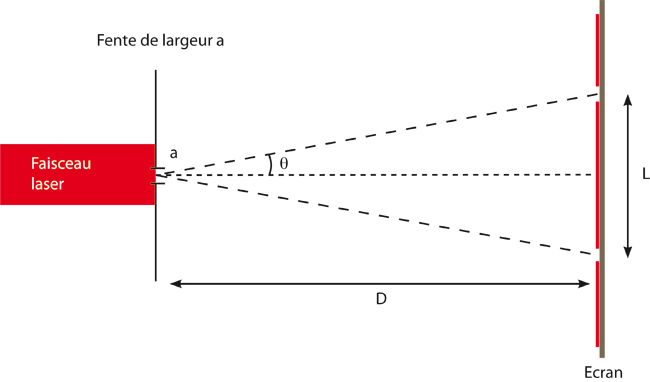
\includegraphics[width=4cm]{laser.png}
		\caption{Diffraction}
	\end{figure}
\end{minipage}
\begin{minipage}[t]{0.46\textwidth}
	Nous reprenons la relation $\lambda=dsin\theta$ et nous déterminons l'angle $\theta=arctan(\frac{\frac{L}{2}}{D})$. La valeur de d étant connue, nous trouvons $\lambda=889.6nm$.
\end{minipage}

Nous déterminons ensuite la largeur de trois fentes différentes à l'aide de la même formule utilisée ci-dessus.
\begin{itemize}
\item Fente 1=0.0926mm
\item Fente 2=0.1728mm
\item Fente 3=0.3703mm
\end{itemize} 


\end{frame}

\begin{frame}
\frametitle{Interférences optiques}

\emph{Observation de figures de diffractions à travers un réseau hexagonal}
\begin{minipage}[t]{0.46\textwidth}
	\begin{figure}
		\centering
		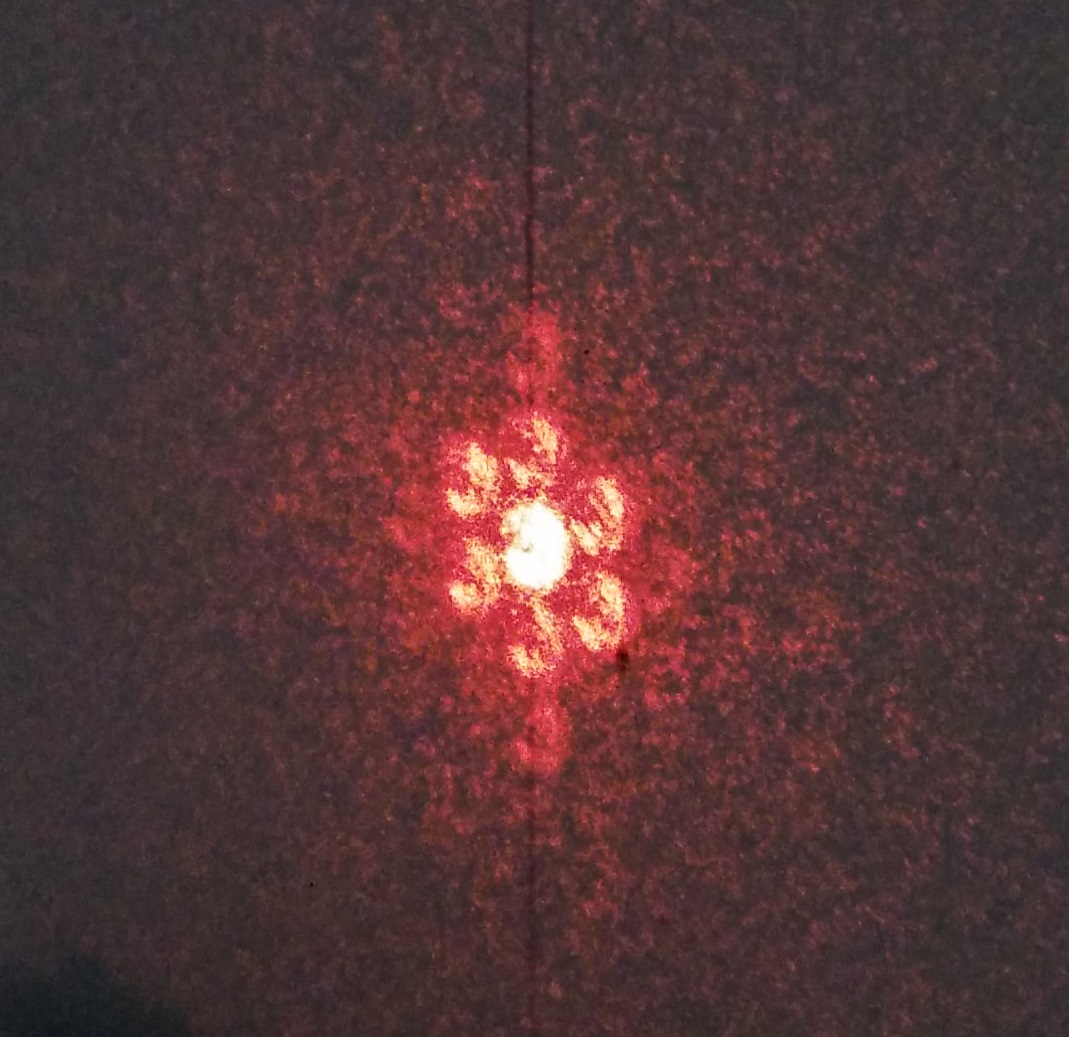
\includegraphics[width=3cm]{hex.jpg}
		\caption{Hex.}
	\end{figure}
\end{minipage}
\begin{minipage}[t]{0.46\textwidth}
	\begin{figure}
		\centering
		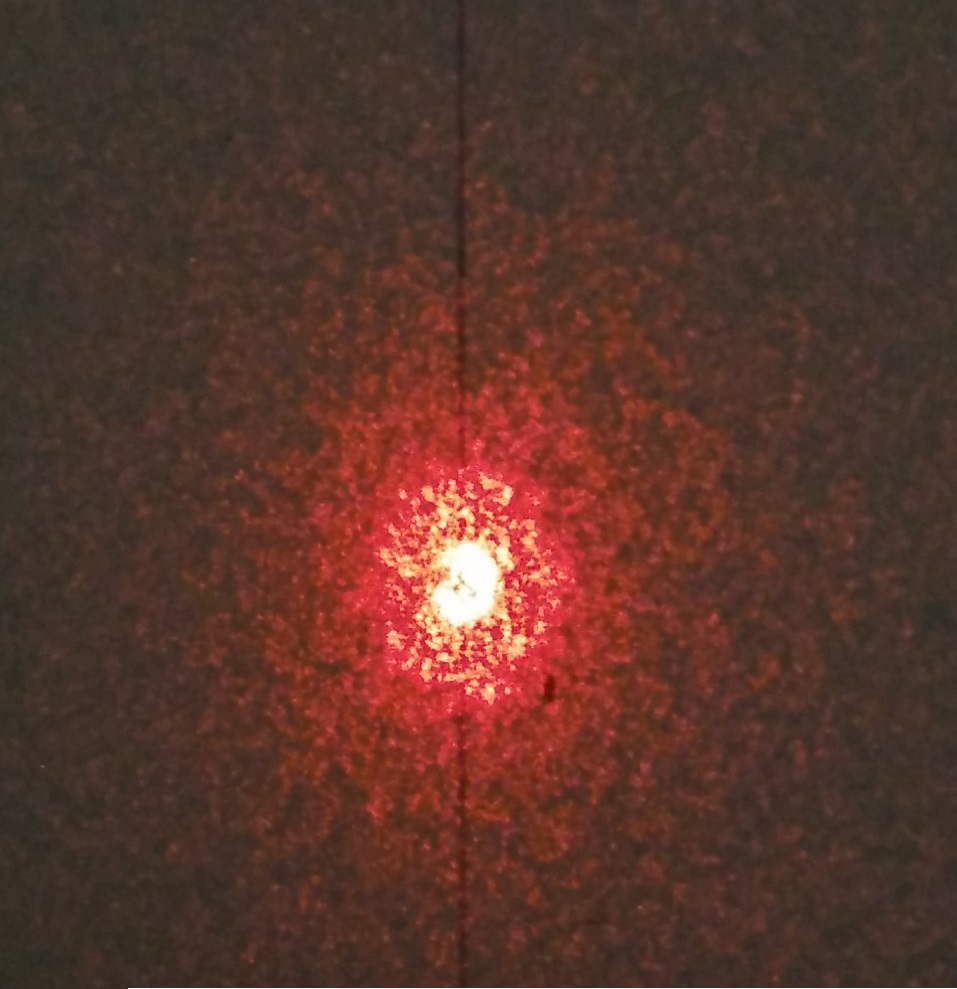
\includegraphics[width=3cm]{polychrist.jpg}
		\caption{Polychrist Hex.}
	\end{figure}
\end{minipage}

\emph{Diffraction à travers un cheveu}
\newline
En considérant que le cheveu agissait comme une fente et en utilisant la même relation, nous avons pu mesuré le diamètre moyen d'un cheveu $d=0.0622mm$


\end{frame}





\end{document}
